\section{Software processes}
\subsection{Software specification}
\subsubsection{Requirements election and analysis}
\begin{itemize}
	\item Beobachtung des existierenden Systems
	\item Absprache mit Nutzern und Entwicklern
	\item Anforderungsanalyse
	\item Entwicklung von Modellen und Prototypen
\end{itemize}
\subsubsection{Requirements specification}
\begin{itemize}
	\item Anforderungen formulieren und dokumentieren
	\item Nuteranforderungen (abstrakt)
	\item Systemanforderungen (detailliert)
\end{itemize}
\subsubsection{Requirements validation}
\begin{itemize}
	\item Umsetzbarkeit
	\item Konsistenz
	\item Vollständigkeit
	\item Fehlerkorrektur 
\end{itemize}
\subsection{Software design and implementation}
\subsubsection{Architectural design}
\begin{itemize}
	\item Systemstruktur
	\item Hauptsächliche Strukturen und Beziehungen
	\item Vertrieb
\end{itemize}
\subsubsection{Database design}
\begin{itemize}
	\item Datenstrukturen
	\item Darstellung in Datenbanken
\end{itemize}
\subsubsection{Interface design}
\begin{itemize}
	\item Eindeutige Interface-Spezifikationen
	\item Kommunikation zwischen Komponenten, ohne Kenntnis der Implementation
\end{itemize}
\subsubsection{Component selection and design}
\begin{itemize}
	\item Suche nach wiederverwendbaren Komponenten
	\item Definiere Veränderungen bei wiederverwendeten Komponenten
	\item Entwerfe neue Komponenten
\end{itemize}
\subsection{Software verification and validation}
\subsubsection{Component testing}
\begin{itemize}
	\item Komponenten durch Entwickler testen
	\item Individuelle Tests, ohne andere Komponenten
\end{itemize}
\subsubsection{System testing}
\begin{itemize}
	\item Komplettes System ist getestet
	\item Fehler von unvorhergesehenen Verwendungen und Interfaces sind behoben
	\item Beweise, dass das System die Anforderungen erfüllt
\end{itemize}
\subsubsection{Customer testing}
\begin{itemize}
	\item Letzte Hürde vor Veröffentlichung
	\item System ist von Nutzer mit echten Daten verwendet worden
	\item Anforderungsprobleme müssen behoben werden
\end{itemize}
\subsection{Software evolution}
Es gibt zwei Wege mit Veränderung umzugehen:
\subsubsection{Change anticipation}
\begin{itemize}
	\item Mögliche Veränderungen vorhersehen
	\item Neustart minimieren
	\item z.B. erst Prototyp erstellen, dann dass ganze Produkt
\end{itemize}
\subsubsection{Change tolerance}
\begin{itemize}
	\item Design berücksichtigt Veränderungen am System
	\item Normalerweise durch schrittweise Entwicklung
	\item Eine kleiner Schritt ist genug um eine Veränderung anzunehmen
\end{itemize}
\subsection{Software development life circle}
\subsubsection{Life cycle phases}
\begin{enumerate}
	\item Initialisierung, Konzept entwickeln, vorläufige Planung, Anforderungsanalyse ($\rightarrow$ Spezifikation)
	\item Design: High-level \& Low-level Design
	\item Implementation
	\item Validierung \& Verifikation
	\item Vertrieb: Veröffentlichung der Anwendung
	\item Erhaltung ($\rightarrow$ Evolution)
	\item Beginne von vorne
	\item Bis Absetzung: Planen der Entfernung der Software (aufräumen \& archivieren) 
\end{enumerate}
\subsection{Software Process Models}
Ein Prozess-Modell ist eine abstrakte Repräsentation der Aktivitäten während des Softwareentwicklungsprozesses um:
\begin{itemize}
	\item Abläufe zu definieren
	\item die Ablaufordnung zu spezifizieren
	\item Phasen zu determinieren: Abläufe, Ziele, Rollen und Methoden 
\end{itemize}
Die Nutzung von Prozess-Modellen führt zu:
\begin{itemize}
	\item einer Richtlinie für die Systementwicklung
	\item einer einheitlichen Ansicht gegenüber logischer und temporärer Planung
	\item besserer Planung
	\item Unabhängigkeit von einzelnen Personen
	\item möglichen Zertifikaten
	\item früherer Erkennung von Fehlern durch Tests 
\end{itemize}
\subsubsection{Wasserfallmodell}
\begin{table}[H]
\caption{Waterfall model}
%\begin{tikzpicture}[main/.style={
%	node distance=10cm,
%	rectangle, minimum size=6mm, rounded corners=3mm,
%	very thick, draw=black!50,
%	top color=white, bottom color=black!20}, node distance=10cm]
%	\node[main] (0) {Requirements analyses \& specification};
%	\node[main, xshift=2cm, yshift=-1.5cm] (1) {System design \& software design};
%	\node[main, xshift=4cm, yshift=-3cm] (2) {Development \& testing};
%	\node[main, xshift=6cm, yshift=-4.5cm] (3) {Integration \& testing};
%	\node[main, xshift=8cm, yshift=-6cm] (4) {Release \& maintenance};
%	\draw[->]
%				(0) edge node[midway, right, xshift=0.5cm] {Specification sheet} (1)
%				(1) edge node[midway, right, xshift=0.5cm] {Software architecture} (2)
%				(2) edge node[midway, right, xshift=0.5cm] {Software} (3)
%				(3) edge (4);
%\end{tikzpicture} 	
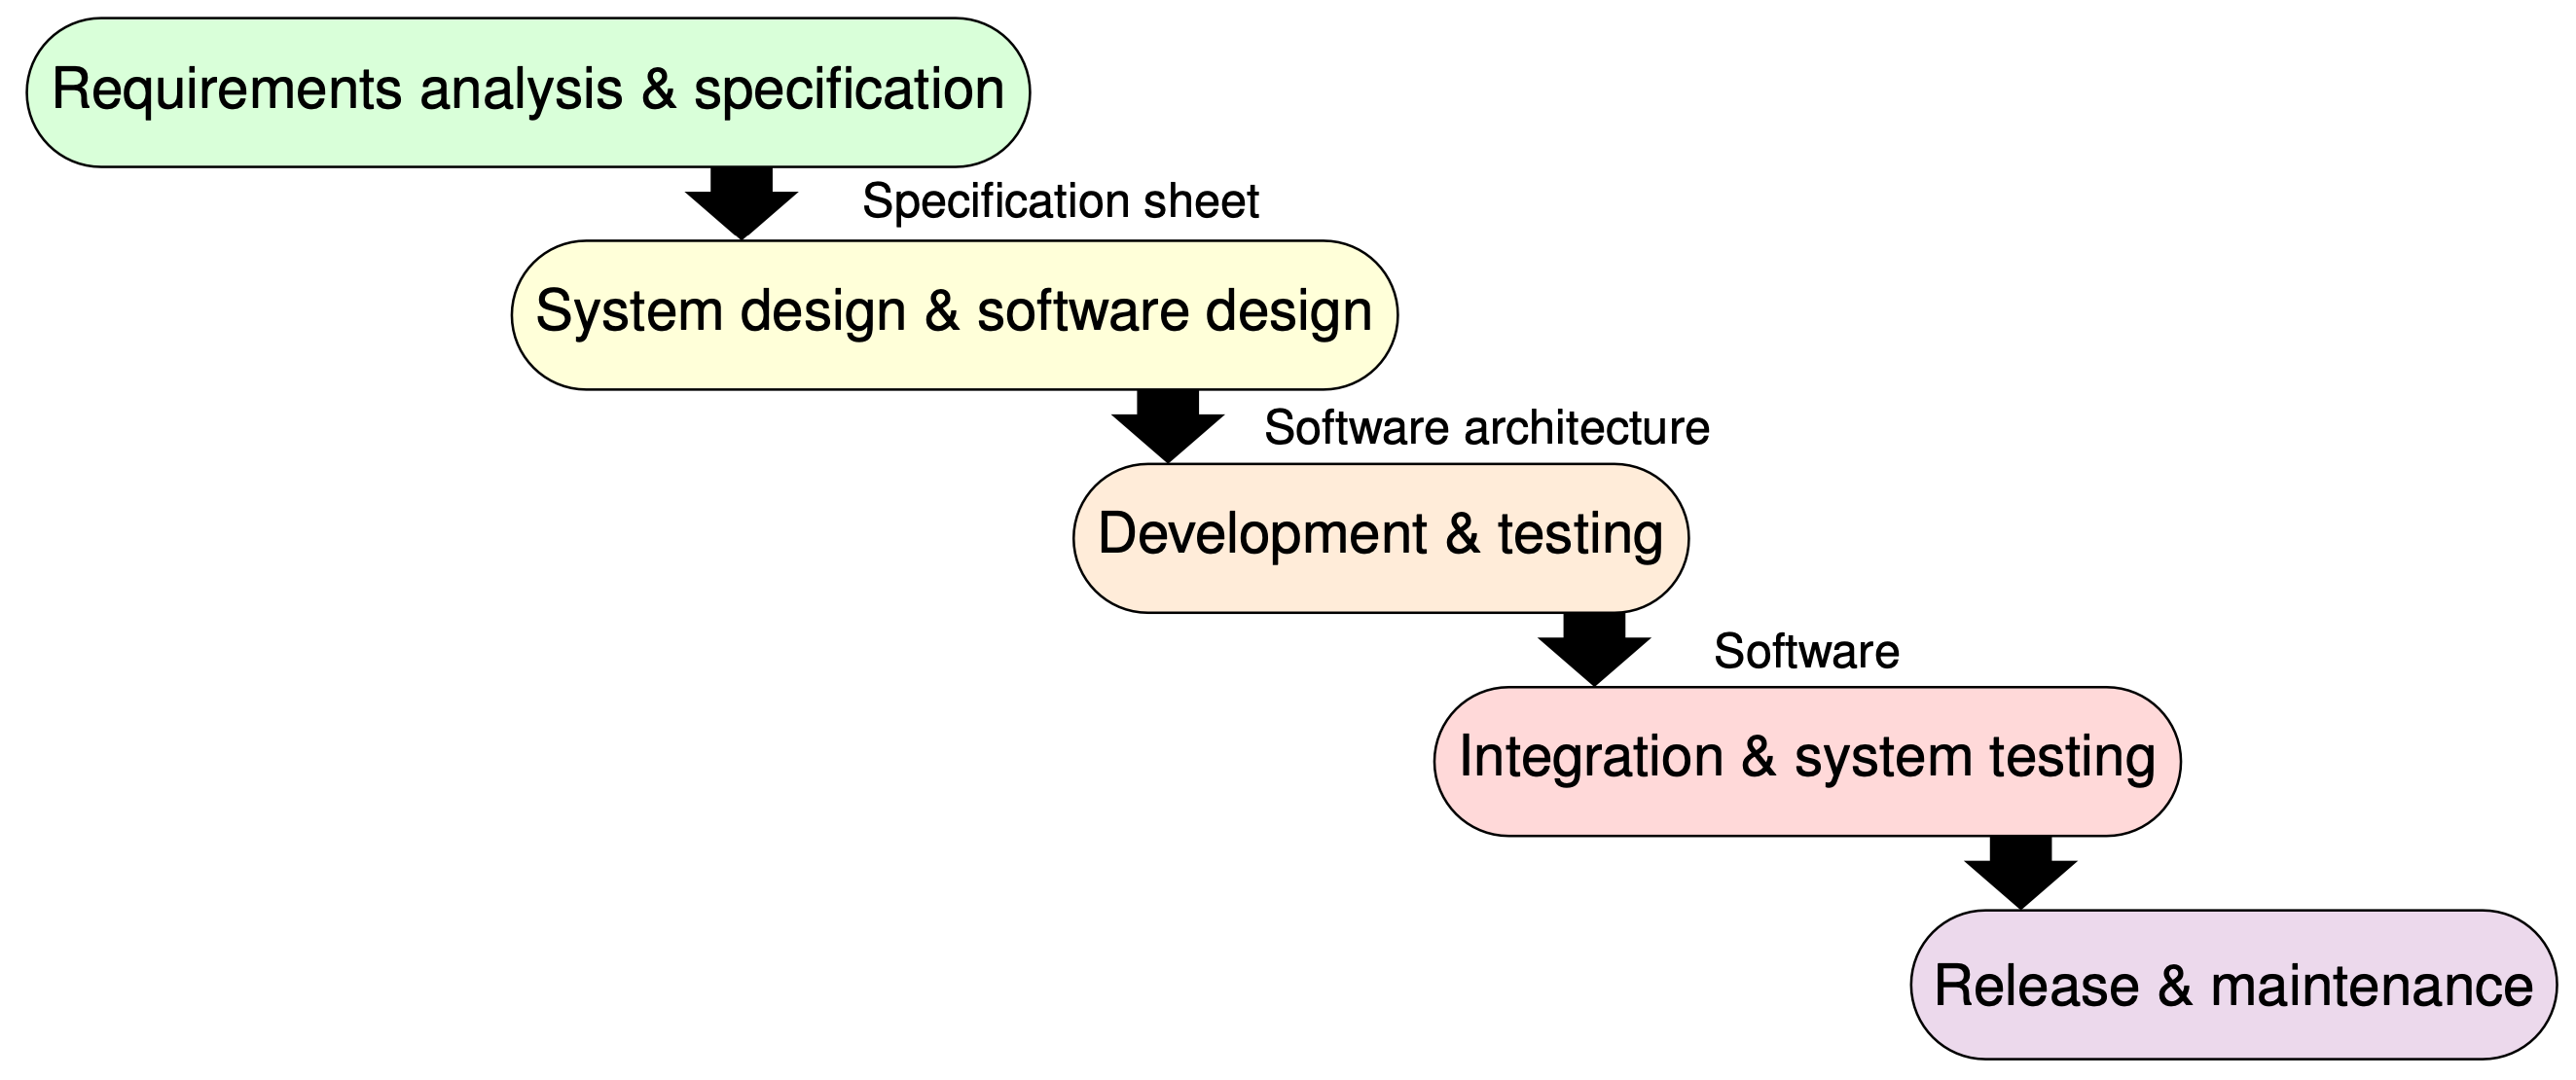
\includegraphics[scale=0.125]{waterfall-model.png}
\end{table}
$\bold{Requirements analyses}$ \& $\bold{specification}$: Projektmanagement beginnt, Probleme und Spezifikationen werden zusammengestellt, Anforderungen definiert und dokumentiert \newline
$\bold{System}$ \& $\bold{software design}$: Entwürfe, Modelle und die Softwarearchitektur werden entwickelt \newline
$\bold{Development}$ \& $\bold{testing}$: Software entwickeln und durch Unit-Tests verifizieren \newline
$\bold{integration}$ \& $\bold{system tests}$: Software Komponenten kombinieren und das Gesamtsystem testen \newline
$\bold{Release}$ \& $\bold{maintenance}$: System installieren, Fehler korrigieren, Software an Altern hindern, neue Anforderungen bearbeiten 
\begin{multicols}{2}
$\bold{Pros}$:
\begin{itemize}
	\item Linearer Prozess
	\item Intuitiv
	\item Einfach verständlich
	\item Top-Down
	\item Planbar
	\item Nicht-Unterbrechbar
\end{itemize}
\columnbreak
$\bold{Cons}$:
\begin{itemize}
	\item Feste Phasen
	\item Frühe Festlegung
	\item Keine Wiederholung
	\item Kein Einbeziehen neuer Anforderungen
	\item Oft unpraktisch
\end{itemize}
\end{multicols}
$\bold{Verwendung}$: \newline
\begin{itemize}
	\item Anforderungen sind einfach zu definieren und ändern sich nicht
	\item Projekt, Budget und Prozess sind vorhersagbar
	\item Strikter Prozess ist notwendig
\end{itemize}
\subsubsection{Improved Waterfall model}
\begin{table}[H]
\caption{Iterative Waterfall model}
%\begin{tikzpicture}[main/.style={
%	node distance=10cm,
%	rectangle, minimum size=6mm, rounded corners=3mm,
%	very thick, draw=black!50,
%	top color=white, bottom color=black!20}, node distance=10cm]
%	\node[main] (0) {Requirements analyses \& specification};
%	\node[main, xshift=2cm, yshift=-1.5cm] (1) {System design \& software design};
%	\node[main, xshift=4cm, yshift=-3cm] (2) {Development \& testing};
%	\node[main, xshift=6cm, yshift=-4.5cm] (3) {Integration \& testing};
%	\node[main, xshift=8cm, yshift=-6cm] (4) {Release \& maintenance};
%	\draw[->]
%				(0) edge node[midway, right, xshift=0.5cm] {Specification sheet} (1)
%				(1) edge node[midway, right, xshift=0.5cm] {Software architecture} (2)
%				(2) edge node[midway, right, xshift=0.5cm] {Software} (3)
%				(3) edge (4)
%				(4) edge [bend left=100] (0)
%				(4) edge [bend left=90] (1)
%				(4) edge [bend left=80] (2)
%				(4) edge [bend left=70] (3);
%\end{tikzpicture}
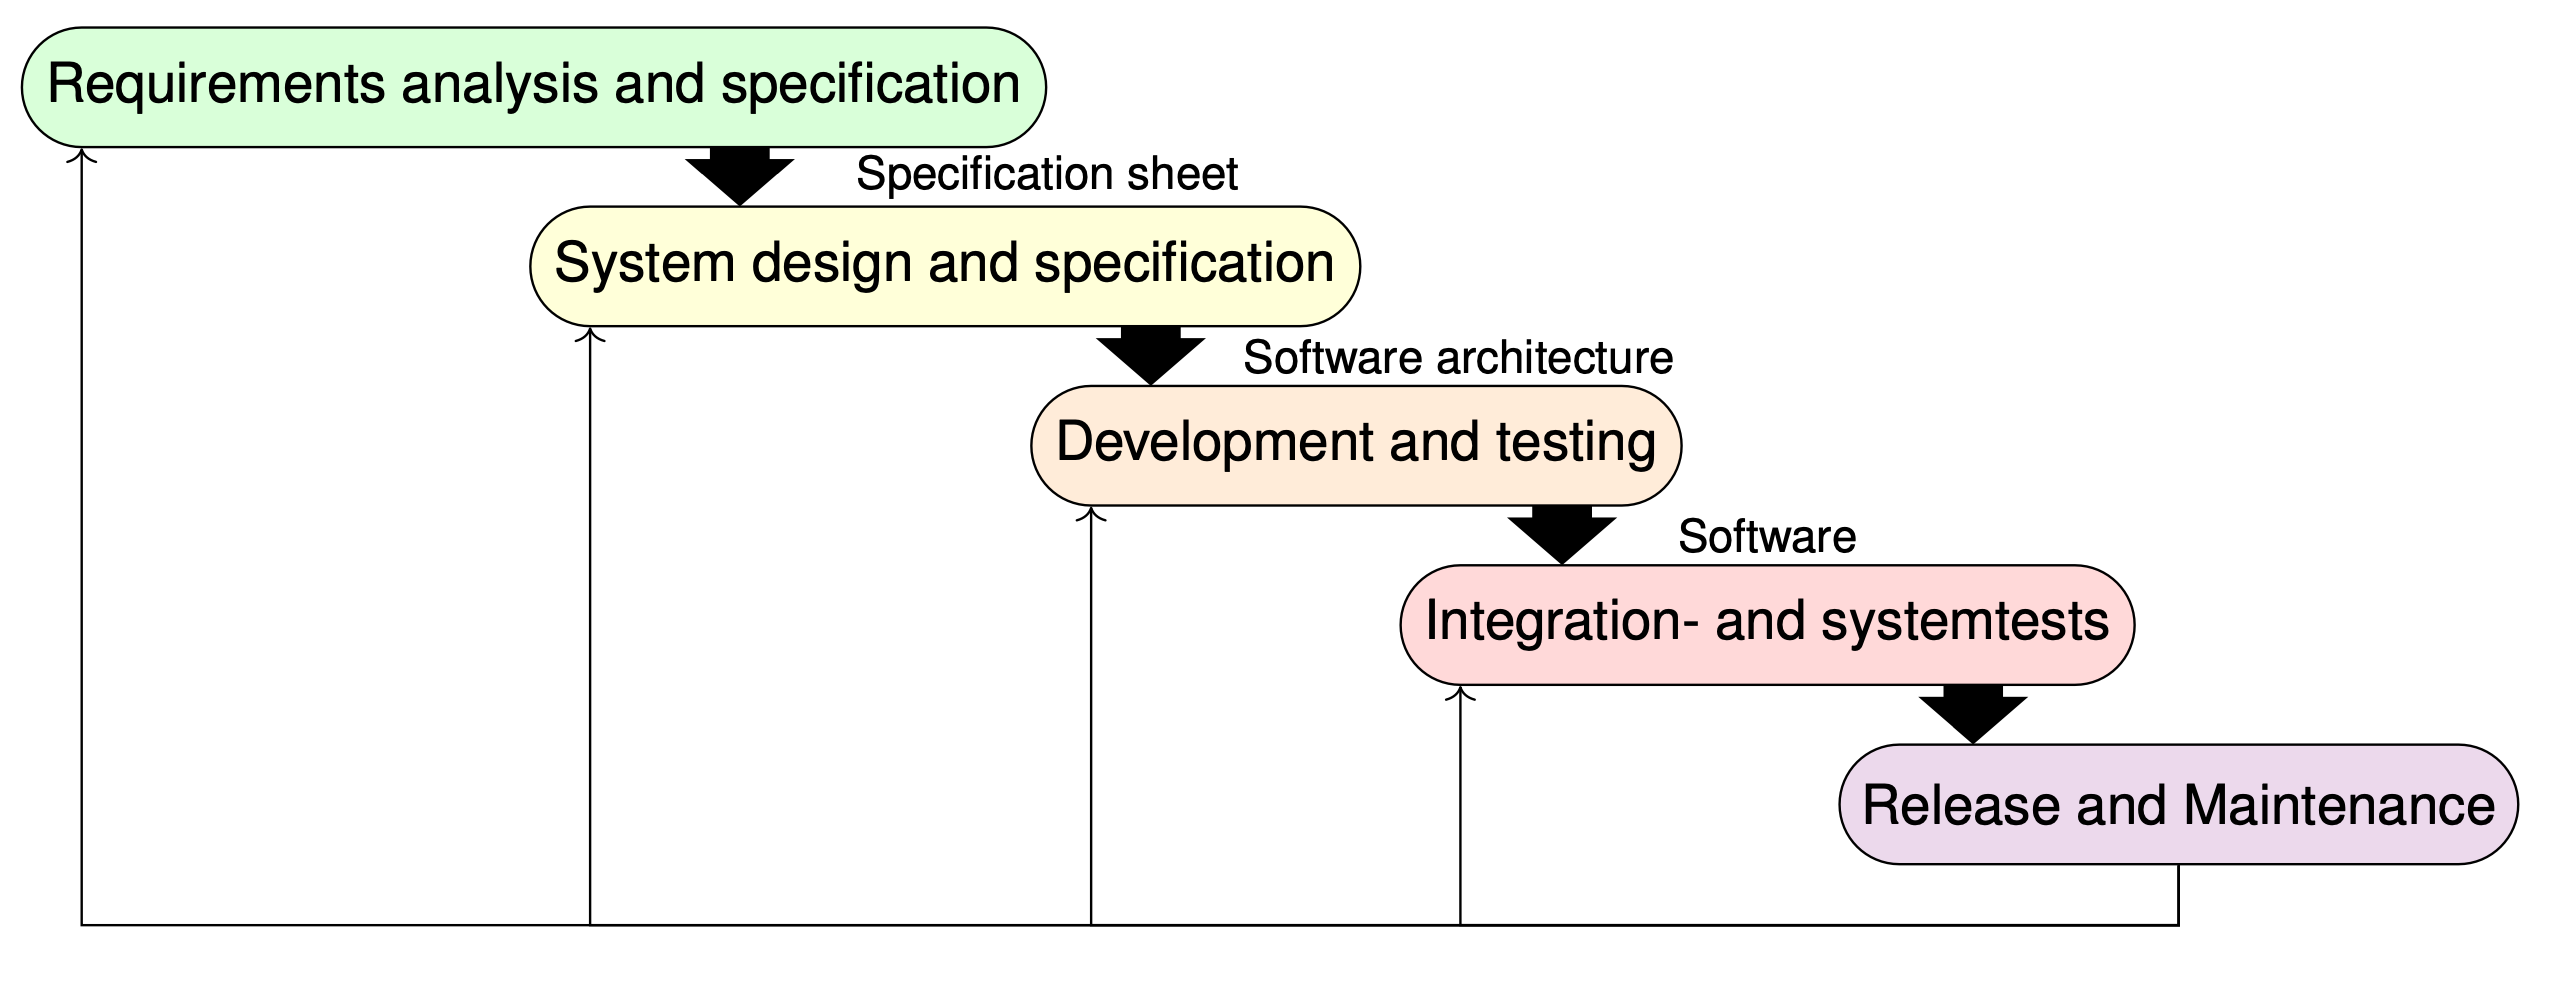
\includegraphics[scale=0.125]{iterative_waterfall-model.png}
\end{table}
\begin{table}[H]
\caption{Incremental Waterfall model}
%\begin{tikzpicture}[main/.style={
%	node distance=10cm,
%	rectangle, minimum size=6mm, rounded corners=3mm,
%	very thick, draw=black!50,
%	top color=white, bottom color=black!20}, node distance=10cm]
%	\node[main] (0) {Requirements analyses \& specification};
%	\node[main, xshift=2cm, yshift=-1.5cm] (1) {System design \& software design};
%	\node[main, xshift=4cm, yshift=-3cm] (2) {Development \& testing};
%	\node[main, xshift=6cm, yshift=-4.5cm] (3) {Integration \& testing};
%	\node[main, xshift=8cm, yshift=-6cm] (4) {Release \& maintenance};
%	\draw[->]
%				(0) edge node[midway, right, xshift=0.5cm] {Specification sheet} (1)
%				(1) edge node[midway, right, xshift=0.5cm] {Software architecture} (2)
%				(2) edge node[midway, right, xshift=0.5cm] {Software} (3)
%				(3) edge (4)
%				(4) edge [bend left=130] (3)
%				(3) edge [bend left=130] (2)
%				(2) edge [bend left=130] (1)
%				(1) edge [bend left=130] (0);
%\end{tikzpicture}
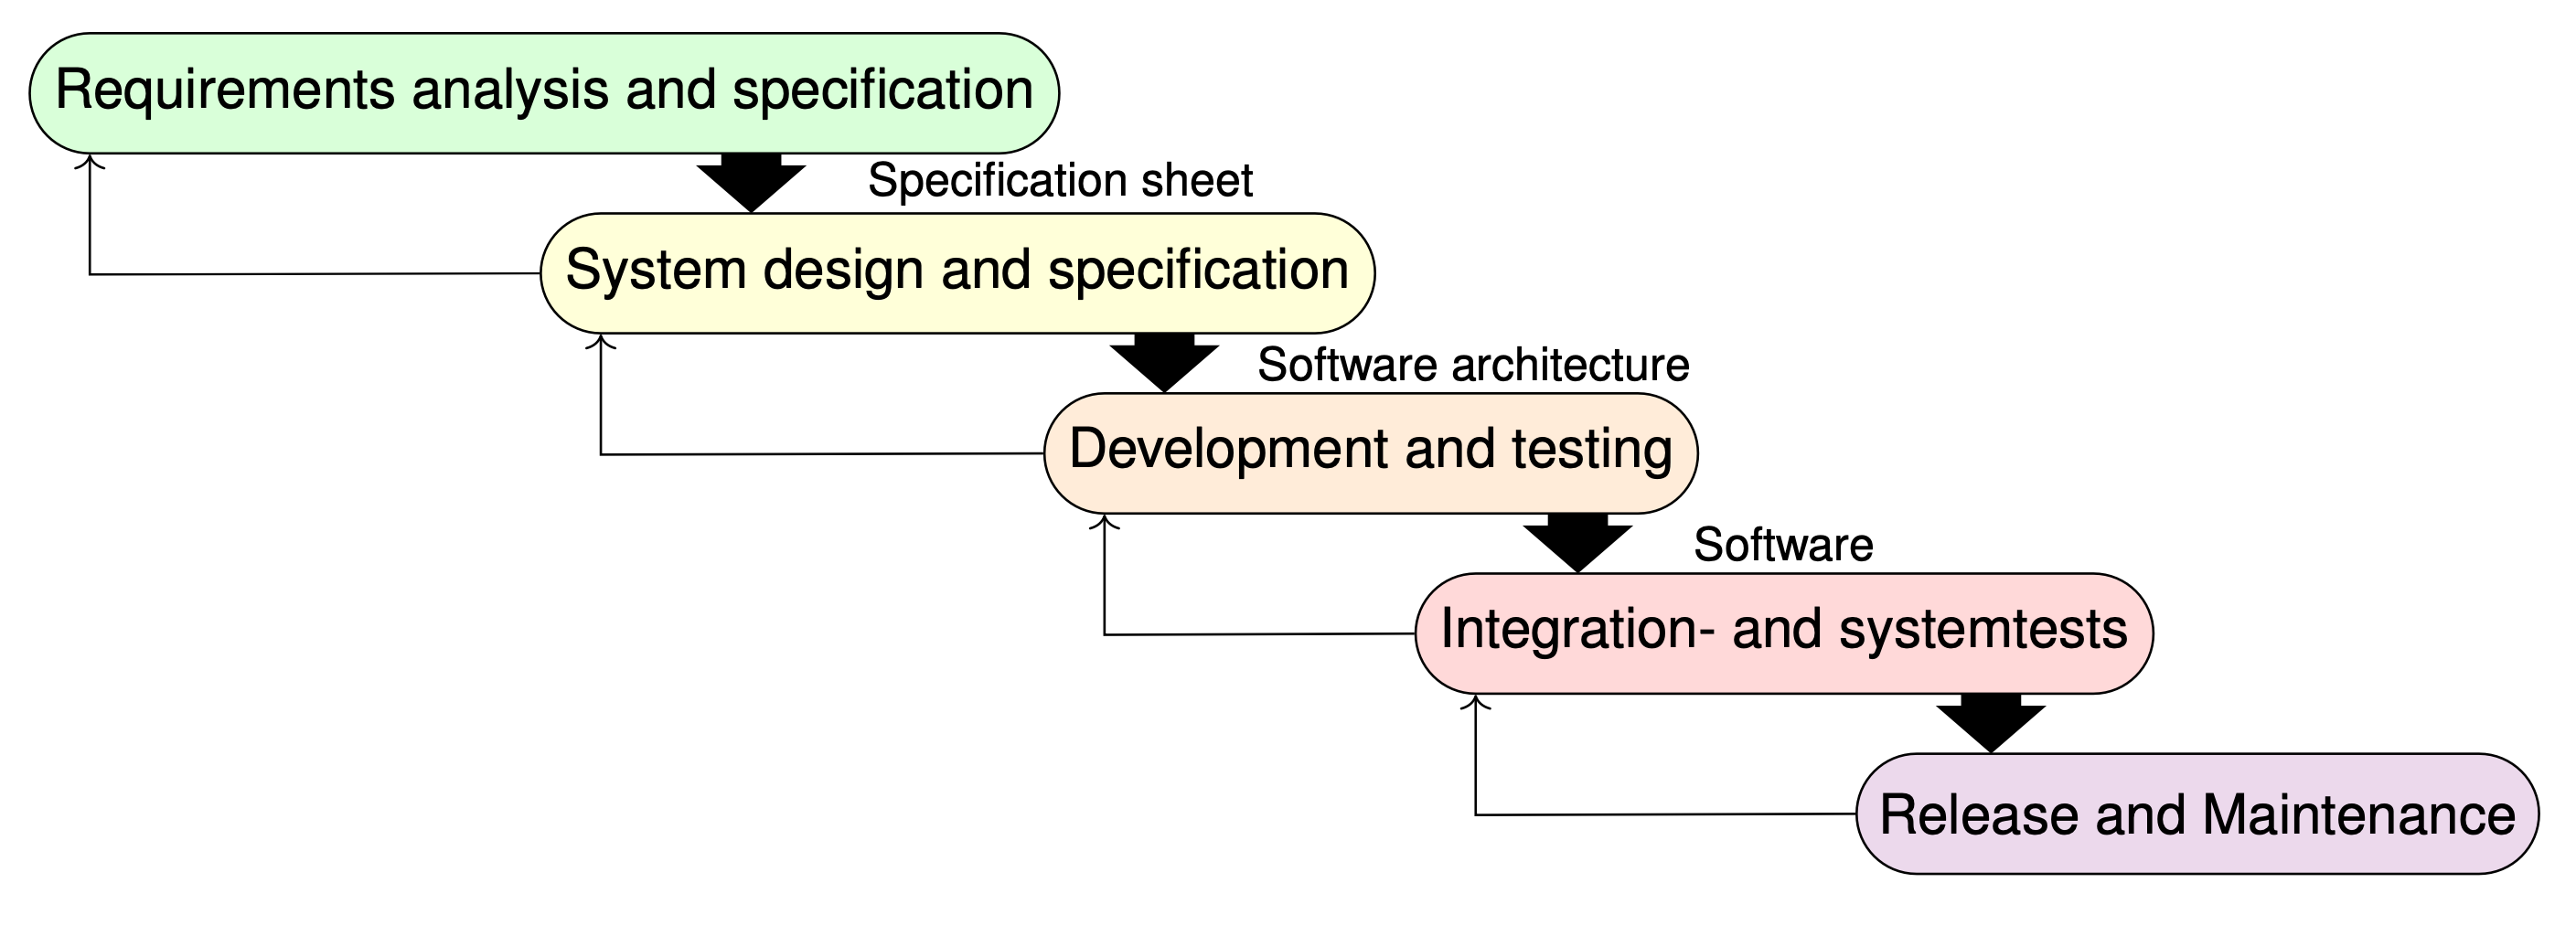
\includegraphics[scale=0.125]{incremental_waterfall-model.png}
\end{table}
\begin{multicols}{2}
$\bold{Pros}$:
\begin{itemize}
	\item Linearer Prozess
	\item Intuitiv
	\item Einfach zu Verstehen
	\item Top-Down
	\item Planbar
	\item Nicht-Unterbrechbar
	\item Wiederholbar
\end{itemize}
\columnbreak
$\bold{Cons}$:
\begin{itemize}
	\item Gefixte Phasen
	\item Frühe Festlegung, aber neue Anforderungen können integriert werden
	\item Veränderte Anforderungen können zu hohen Kosten führen
	\item Struktur tendiert abzubauen
\end{itemize}
\end{multicols}
$\bold{Verwendung}$: \newline
\begin{itemize}
	\item Anforderungen sind einfach definiert
	\item Nur kleine Änderungen können erscheinen und sind im Budget mit eingerechnet
	\item Projekt, Budget und Prozess sind vorhersagbar
	\item Strikter, aber leicht flexibler Prozess ist notwendig 
\end{itemize}
\subsubsection{V-Modell}
\begin{table}[H]
\caption{V-model}
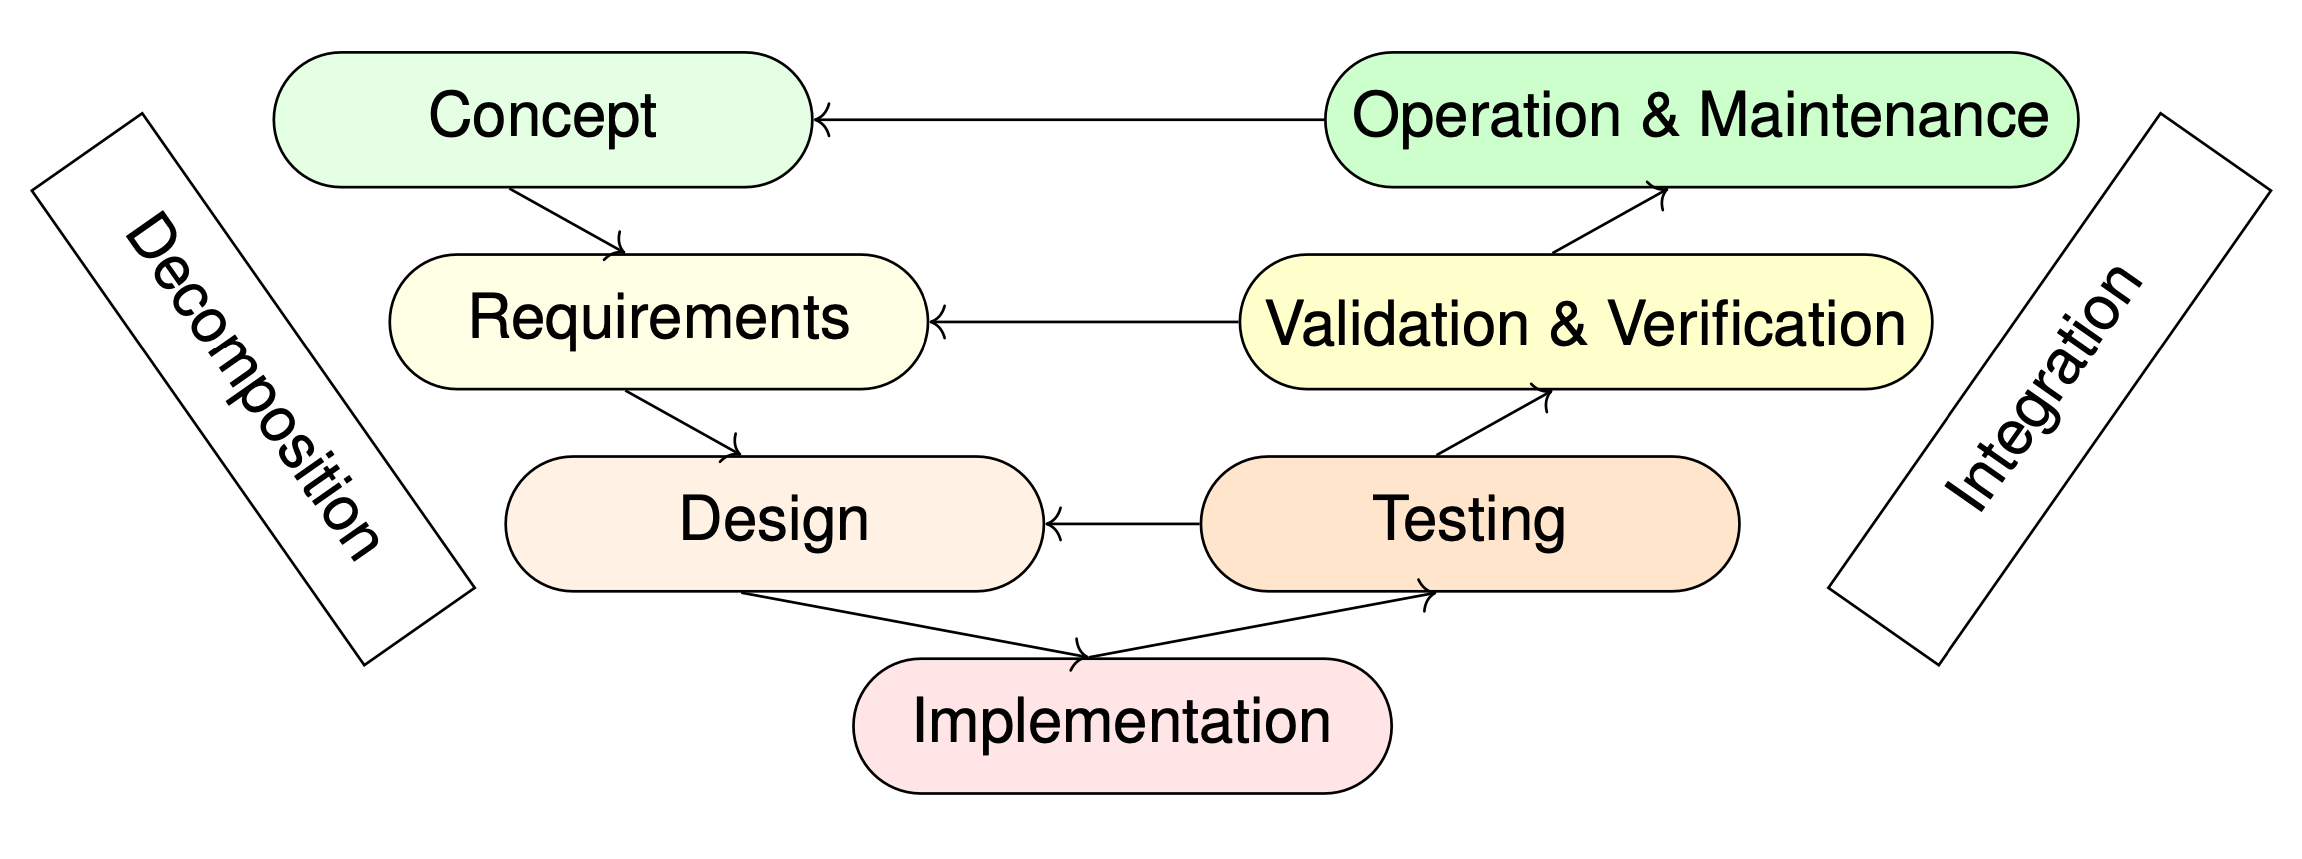
\includegraphics[scale=0.15]{v-model.png}
\end{table}
\begin{table}[H]
\caption{V-model XT}
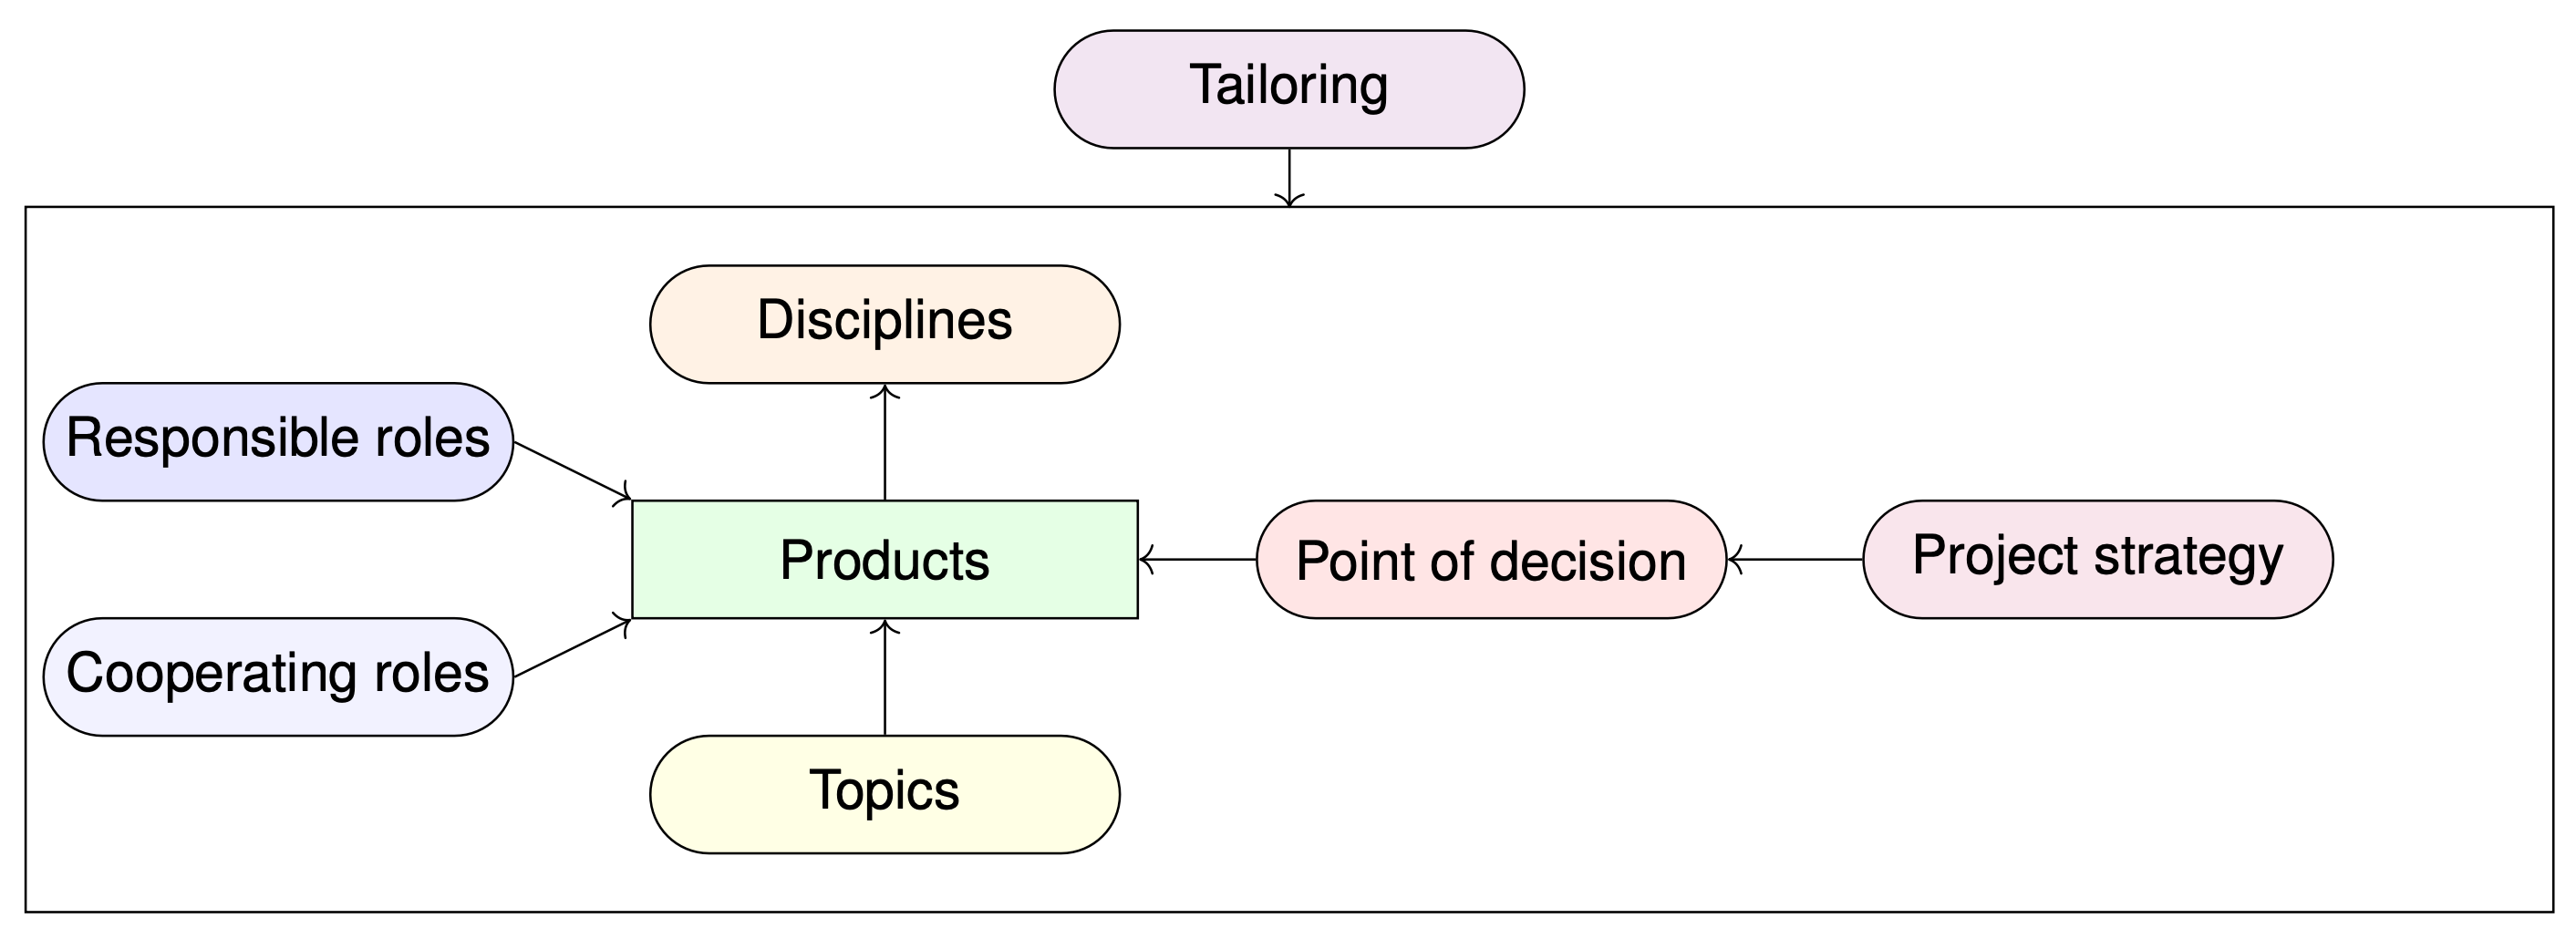
\includegraphics[scale=0.125]{v-model_XT.png}
Jedes Produkt geht durch vordefinierte Zustände
\begin{center}
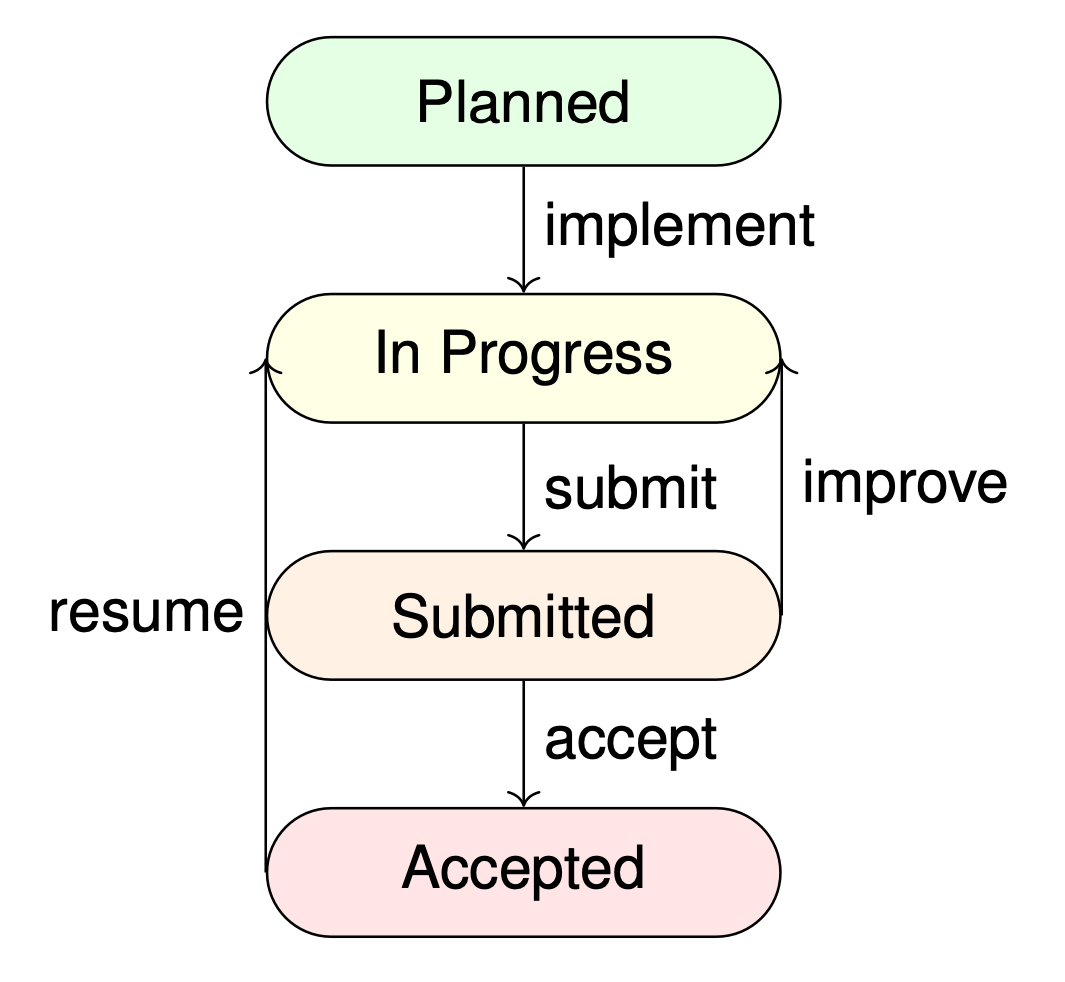
\includegraphics[scale=0.125]{v-model_XT_states.png}	
\end{center}
\end{table}
\begin{multicols}{2}
$\bold{Pros}$:
\begin{itemize}
	\item Bei großen und komplexen Systemen anwendbar
	\item detaillierte Spezifikationen, Rollendefinitionen und Ergebnisstrukturen
	\item Qualitätsorietiert
\end{itemize}
\columnbreak
$\bold{Cons}$:
\begin{itemize}
	\item Großer Overhead bei kleinen Projekten
	\item Testphase begint relativ spät
	\item Strikte Phasen
	\item Teilnehmer müssen geschult sein, um Modell zu folgen
\end{itemize}
\end{multicols}
$\bold{Verwendung}$: \newline
\begin{itemize}
	\item Softwareentwicklung in Behörden
	\item Sicherheitsrelevante Projekte 
\end{itemize}
\subsubsection{Wiederverwendungsansatz}
\begin{table}[H]
\caption{Reuse-oriented approach}
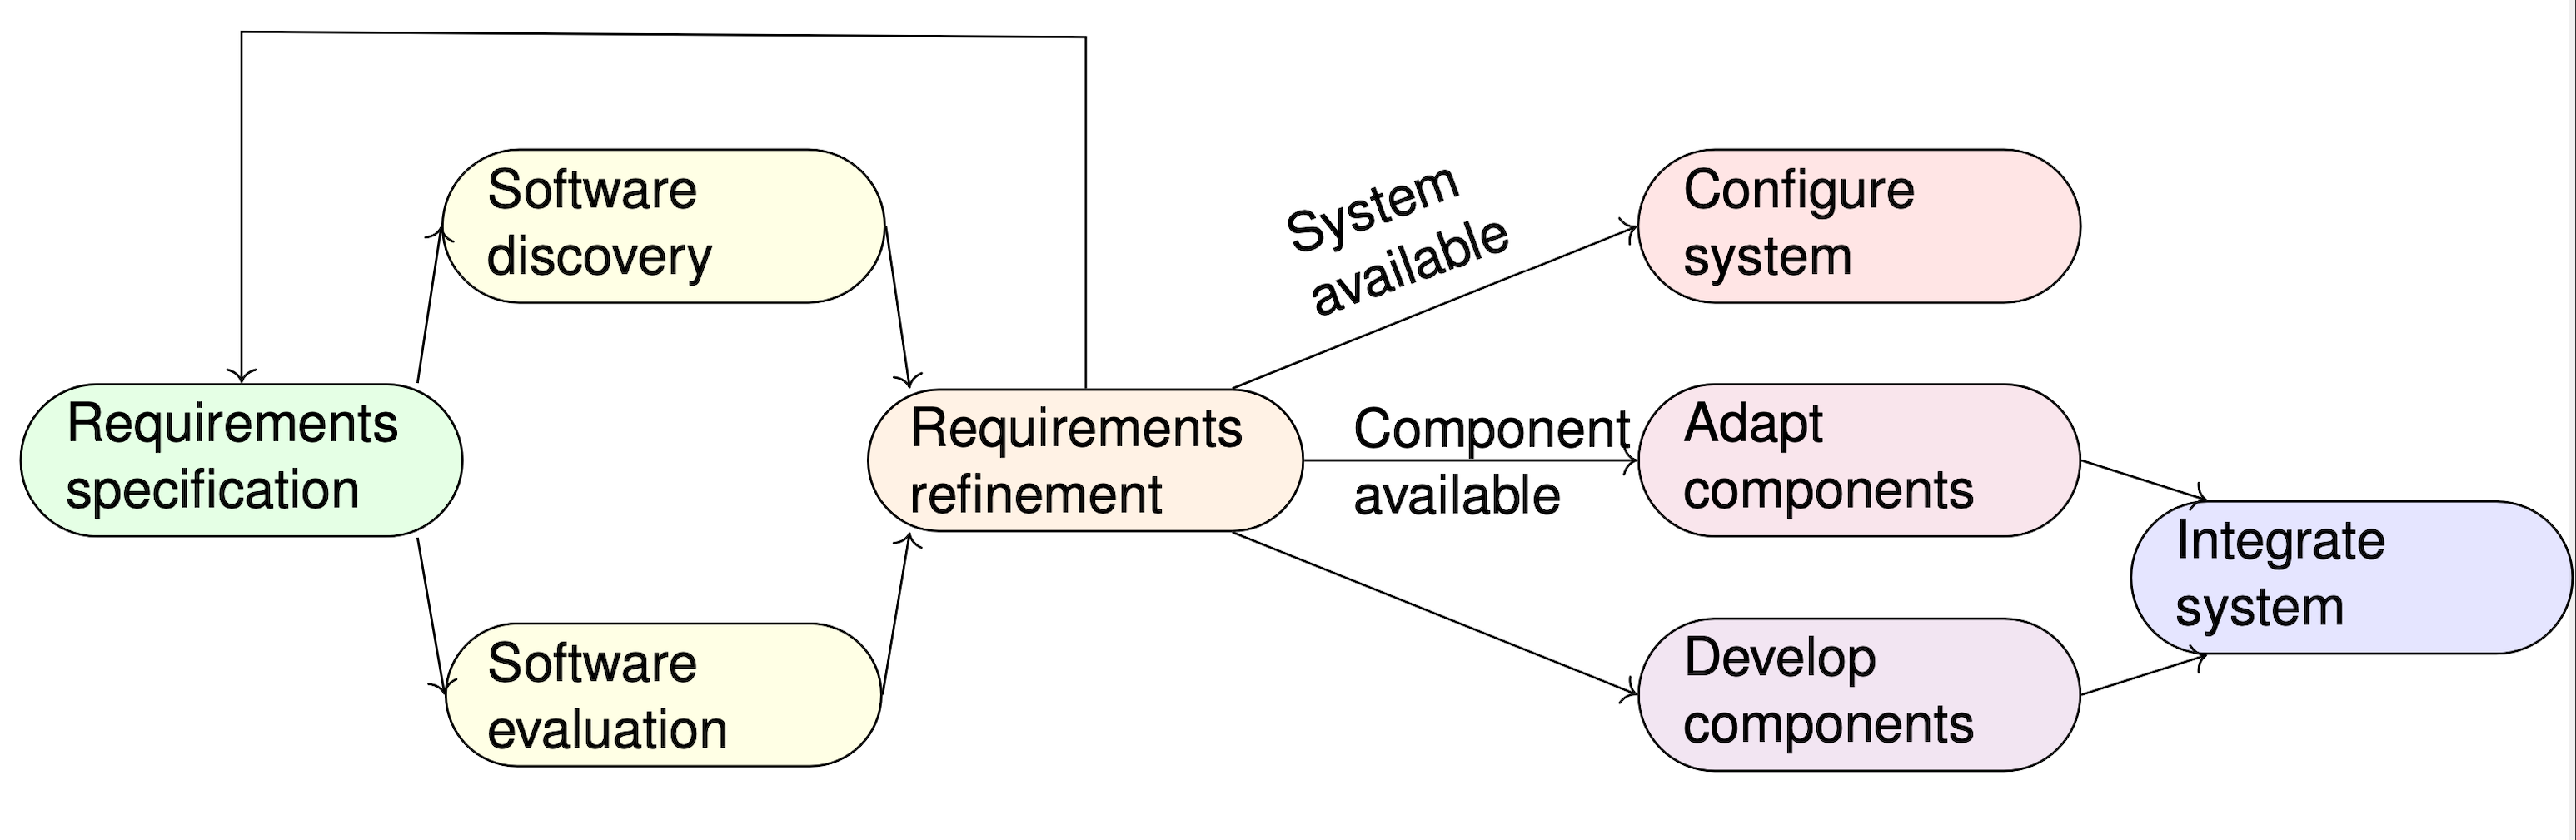
\includegraphics[scale=0.125]{reuse-oriented_approach.png}
\end{table}
\begin{multicols}{2}
$\bold{Pros}$:
\begin{itemize}
	\item Reduziert Kosten und Risiken
	\item Schnellere Verteilung
\end{itemize}
\columnbreak
$\bold{Cons}$:
\begin{itemize}
	\item Kompromisse in den Anforderungen
	\item System könnte echte Nutzerbedürfnisse nicht erfüllen
	\item Kein oder limitierte Kontrolle über Systemevolution
\end{itemize}
\end{multicols}
$\bold{Verwendung}$:
\begin{itemize}
	\item Webanwendungen
	\item Collection of objects or packages
	\item Konfigurierbare stand-alone Softwaresysteme
\end{itemize}
\subsubsection{Agiles Modell}
\begin{table}[H]
\caption{Agile model}
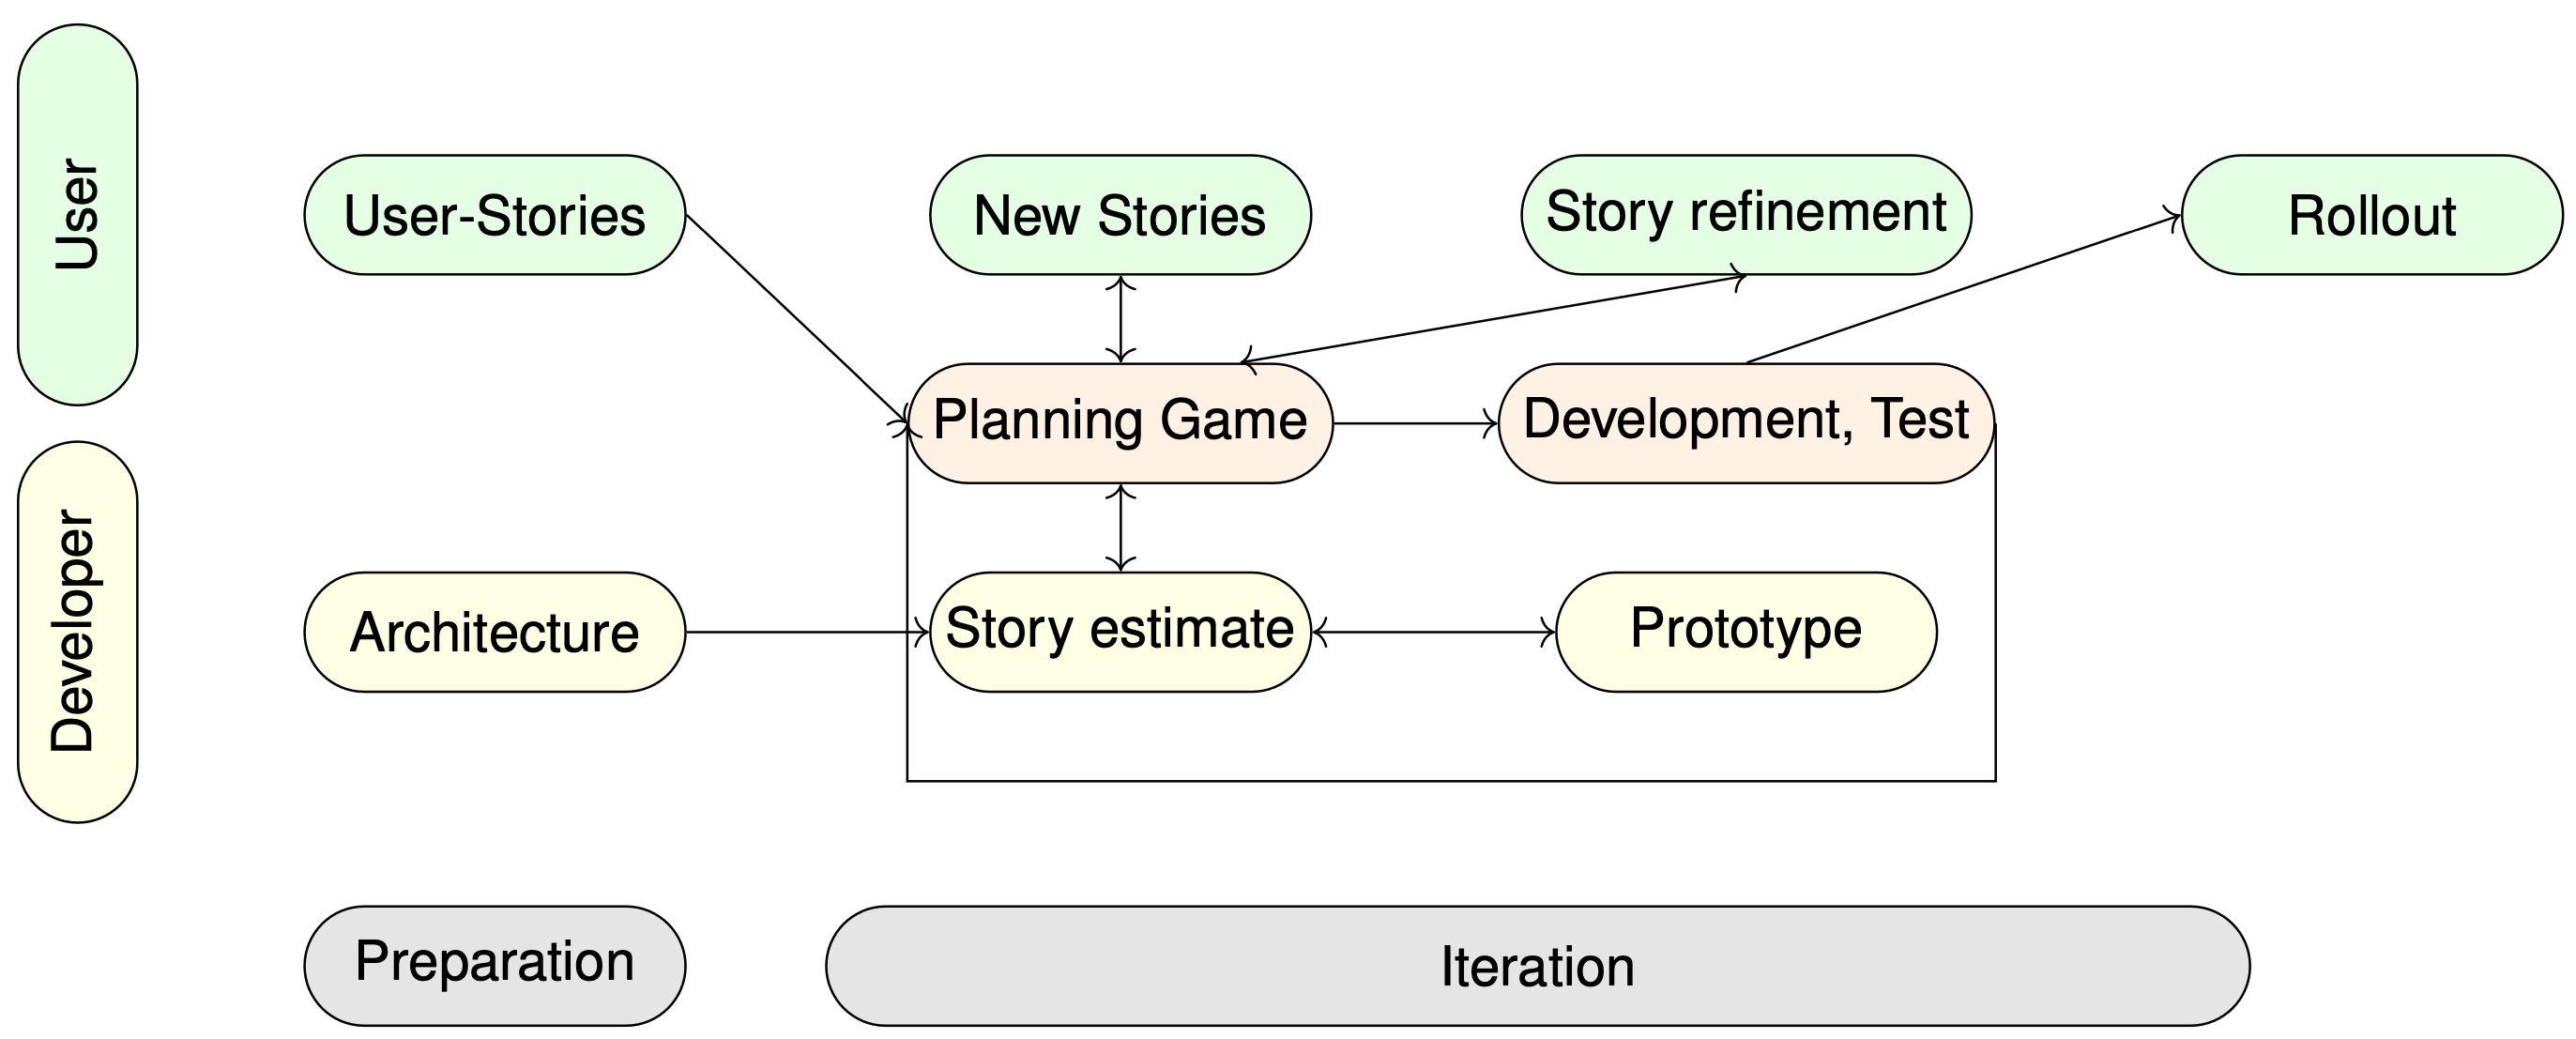
\includegraphics[scale=0.125]{agile_model.png}
\end{table}
\begin{multicols}{2}
$\bold{Pros}$:
\begin{itemize}
	\item Begrenzter bürokratischer Aufwand
	\item Flexible Rollen
	\item so wenig Dokumentation wie nötig
	\item besseres Kosten/Nutzen Verhältnis
	\item Bessere Code-Qualität
\end{itemize}
\columnbreak
$\bold{Cons}$:
\begin{itemize}
	\item Ganzes Team muss den Regeln folgen
	\item Projektergebnis nicht vorhersehbar
\end{itemize}
\end{multicols}
$\bold{Verwendung}$:
\begin{itemize}
	\item Große, komplexe sowie kleine Systeme
	\item Projekte die Prototypen erfordern 
\end{itemize}
\subsection{Change Management}
\subsubsection{Prototyp}
\begin{table}[H]
\caption{Prototyping}
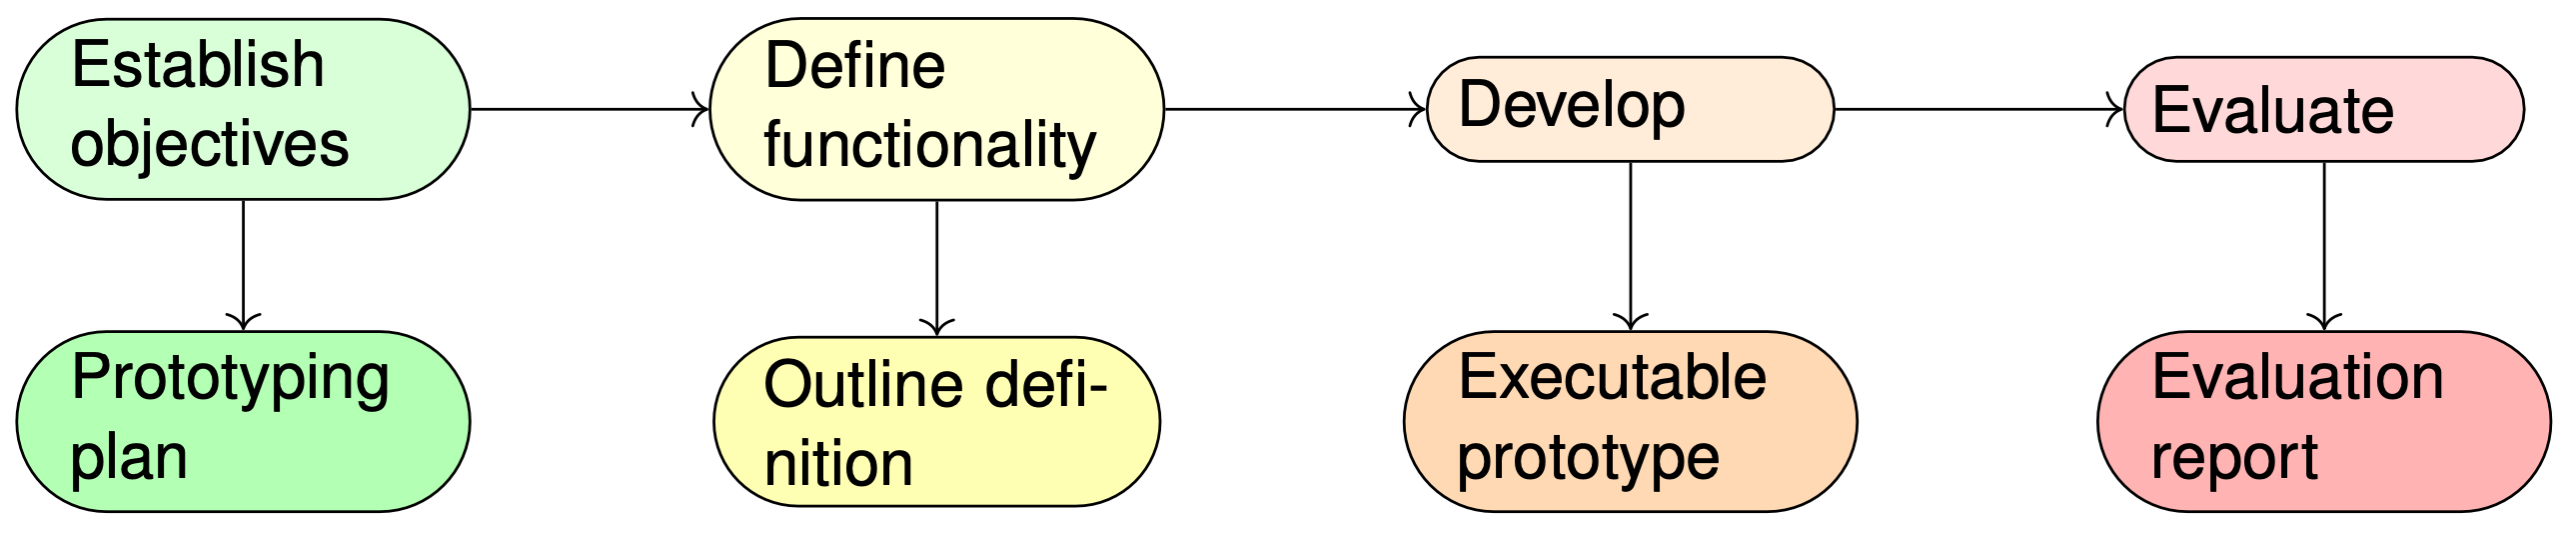
\includegraphics[scale=0.125]{prototyping.png}
\end{table}
\begin{multicols}{2}
$\bold{Pros}$:
\begin{itemize}
	\item Kunde gibt Priorität der Anwendung vor
	\item Software kann sofort verwendet werden
	\item Kunde erlangt Erfahrung mit dem System
	\item Kunde kann Anforderungen für spätere Schritte abgeben
	\item Veränderungen sind einfach umzusetzen
	\item Die wichtigsten Systemteile werden am häufigsten gestet 
\end{itemize}
\columnbreak
$\bold{Cons}$:
\begin{itemize}
	\item Softwarebasis kann ohne detaillierte Anforderungen nicht identifiziert werden
	\item Kann mit organisatorischen Strukturen in Konflikt geraten (z.B. Verträge)
	\item Unbrauchbar um existierende Systeme zu ersetzen
\end{itemize}
\end{multicols}
\subsubsection{Schrittweise Veröffentlichung}
\begin{table}[H]
\caption{Incremental delivery}
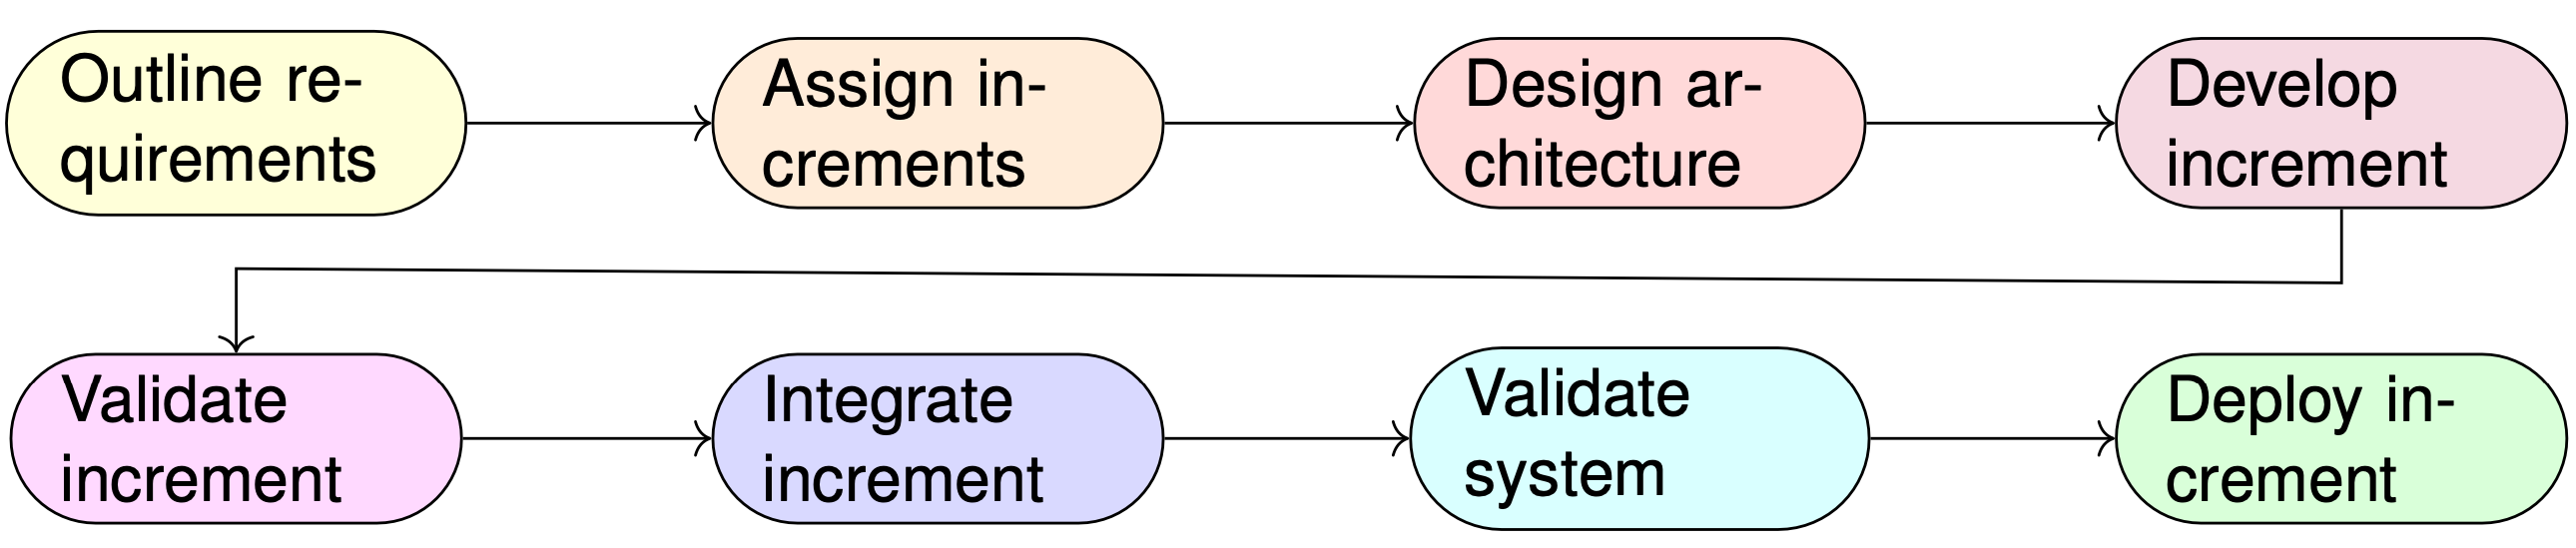
\includegraphics[scale=0.125]{incremental_delivery.png}
\end{table}

























